\section{Kết quả đạt được}
    Nhóm đã hiện thực được thuật toán, xây dựng hoàn chỉnh hệ thống website bao gồm cả hệ cơ sở dữ liệu và quản lý khảo sát người dùng. Hệ thống gồm một số chức năng như làm một số bài kiểm ra, đưa ra gợi ý theo thuật toán cho người dùng, tin tức, chức năng quản lý giành cho nhóm phát triển. Sau khi hiện thực, nhóm tiến hành một cuộc khảo sát nhỏ trên 100 sinh viên ngẫu nhiên và thu được kết quả khả quan khi 69,7\% gợi ý được các sinh viên cảm thấy phù hợp. Việc phát triển đồ án này hy vọng sẽ giải quyết được tình trạng vô cùng nhức nhối đã được nêu lên ở phần thực trạng, có thể đóng góp một phần nhỏ vào việc phát triển bền vững hơn trong tương lai.
    
    \begin{figure}[H]
        \centering
        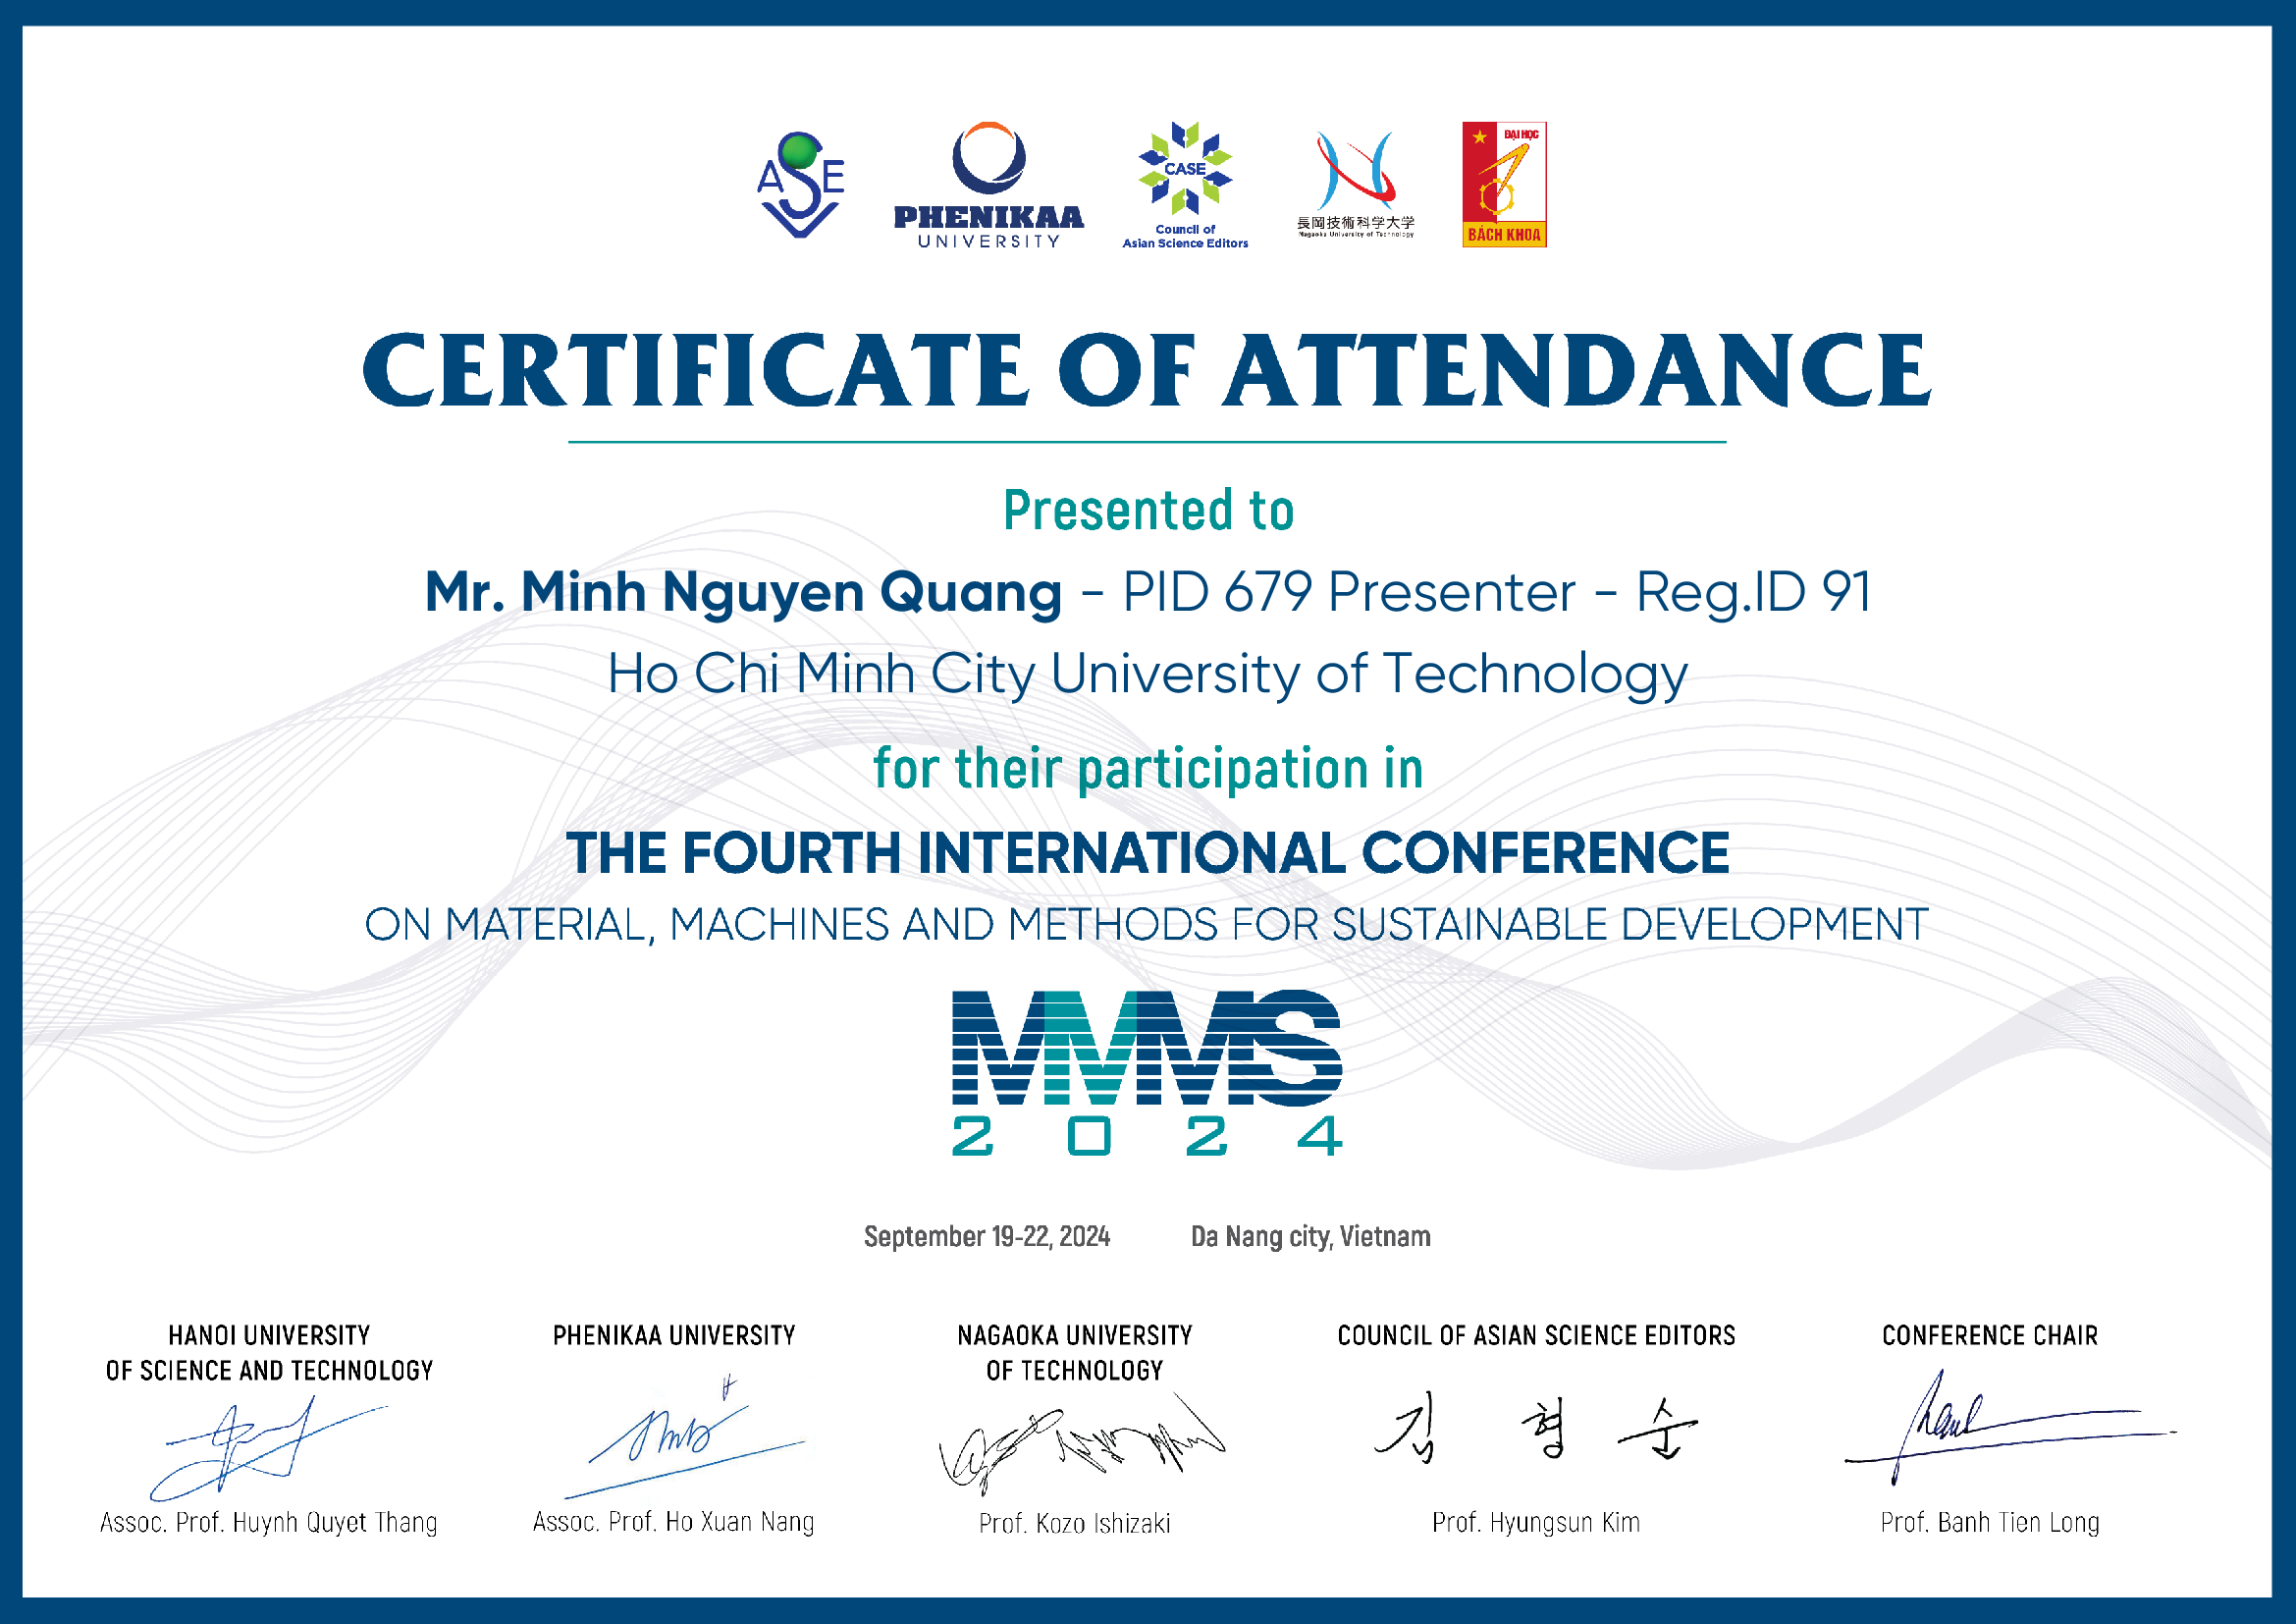
\includegraphics[width=0.8\linewidth, height=0.3\textheight]{images/present.png}
        \vspace{0.6cm}
        \caption{Chứng nhận đã thuyết trình ở hội nghị MMMS2024 của đề tài}
    \end{figure}

    \begin{figure}[H]
        \centering
        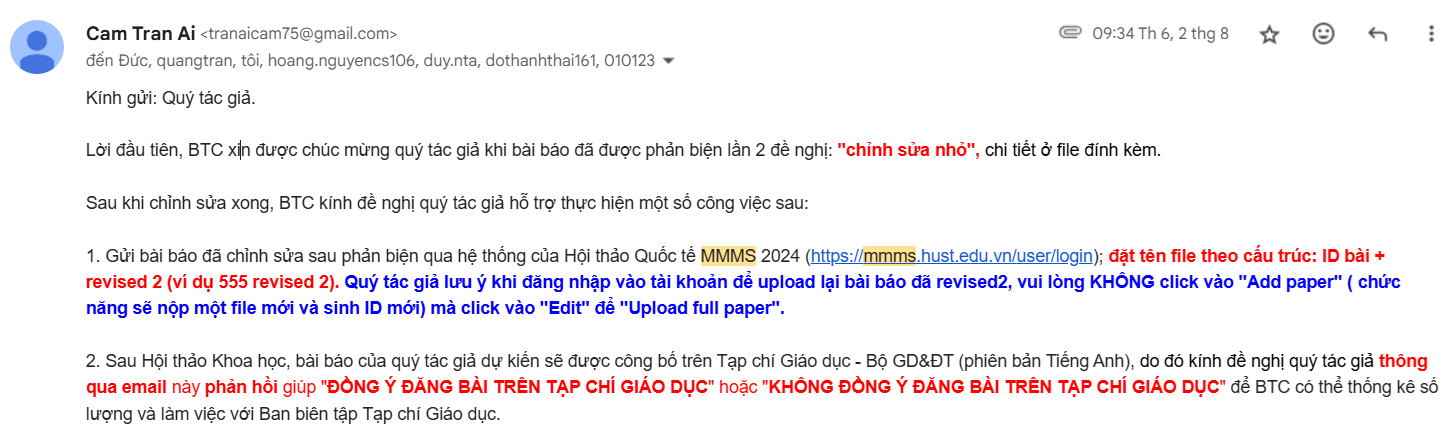
\includegraphics[width=0.8\linewidth]{images/email.png}
        \vspace{0.6cm}
        \caption{Chứng nhận đã được chấp thuận thông qua ở hội nghị MMMS2024 của đề tài}
    \end{figure}
    

    Đồ án cũng đã được chấp nhận công bố trên Tạp chí Giáo Dục Việt Nam bản tiếng anh(VietNam Journal of Education) và đã thuyết trình tại hội nghị trong hội nghị MMMS2024 - the fourth international conference on material, machine, and method for sustainable development. Đây cũng là một sự công nhận với những gì nhóm đã cố gắng nghiên cứu và thực hiện, hy vọng đồ án có thể được kế thừa và phát triển tốt hơn và đạt được mục tiêu mà nhóm đề ra về hỗ trợ mọi người tìm ra lý do để sống - ikigai của riêng bản thân mình.